\subsection{Định luật I}
\begin{frame}
    \frametitle{Định luật quán tính}
    \begin{tcolorbox}[colback=blue!10, colframe=blue!50!black, title= Định luật I]
        Một vật thể sẽ chuyển động với vận tốc không đổi (có thể bằng không) cho tới khi chịu tác động của vật khác.
    \end{tcolorbox}
    \begin{tcolorbox}[colback=blue!10, colframe=blue!50!black, title=Hệ quy chiếu quán tính]
        Tồn tại một hệ quy chiếu sao cho một vật không chịu tác động của vật khác sẽ chuyển động với vận tốc không đổi (có thể bằng 0).
    \end{tcolorbox}
\end{frame}
\subsection{Định luật II}
\begin{frame}
    \frametitle{Định lượng cho sự tương tác}
    \begin{itemize}
        \item Động lượng của một vật chịu tác động của các vật khác sẽ thay đổi.
        \item Sự thay đổi này có thể diễn ra liên tục. 
        \item Có thể coi quá trình tương tác liên tục này là một chuỗi va chạm liên tục giữa các vật : \[\Delta\mathbf{p}=\Delta \mathbf{p}_1 +\Delta\mathbf{p}_2 +\cdots.\]
        \item Định lượng khái niệm tương tác vật lý:
        \[\mathbf{F}=\lim_{\Delta t\to 0}\frac{\Delta\mathbf{p}}{\Delta t}.\] 
        
    \end{itemize}
\end{frame}
\begin{frame}
    \frametitle{Định luật II}
    \vspace{-5pt}

    \begin{tcolorbox}[colback=blue!10, colframe=blue!50!black, title=Lực]
        Biến thiên động lượng theo thời gian của vật thể bằng lực tác dụng lên vật thể:
        \begin{equation}
            \mathbf{F}=\frac{\text{d}\mathbf{p}}{\text{d}t}.
        \end{equation}
    \end{tcolorbox}
    Phát biểu này đúng trong các hệ quy chiếu quán tính với sự thừa nhận lực mà một vật thể tác dụng lên một vật thể khác là bất biến trong mọi hệ quy chiếu.\newline
    Với giới hạn khối lượng không đổi,
    \vspace{-2pt}

    \begin{equation}
        \mathbf{F}=m\mathbf{a}.
    \end{equation}
    Thoả mãn định luật I: Trong một hệ quy chiếu quán tính, \(\mathbf{a}=\mathbf{0}\) khi \(\mathbf{F}=\mathbf{0}\).
\end{frame}
\begin{frame}
    \frametitle{Định luật II Newton và nguyên lý tương đối Galilei}
    Nguyên lý tương đối Galilei:\emph{ Các phương trình động lực học không biến đổi khi chuyển từ hệ quy chiếu quán tính này sang hệ quy chiếu quán tính khác.}
    \begin{columns}
        \begin{column}{0.5\textwidth}
            \vspace{-5pt}

            \begin{figure}
                \centering
                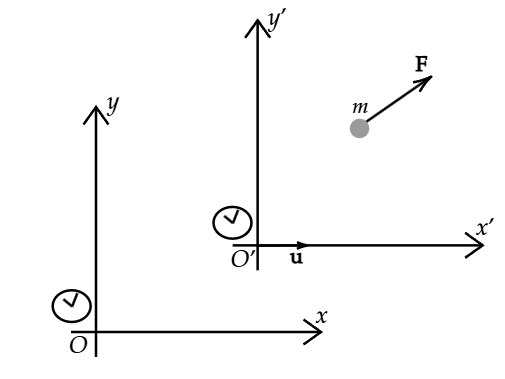
\includegraphics[width=6cm, height=4cm]{Slides/Figure/Galilei.png}
                \caption{\(\mathbf{F}=m\mathbf{a}=m\mathbf{a'}\)}
            \end{figure}
        \end{column}
        \begin{column}{0.5\textwidth}
            \vspace{5pt}

            Không gian tương đối: khoảng cách giữa hai sự kiện phụ thuộc vào hệ quy chiếu 
            \[x'_2 -x'_1 =(x_2 -x_1)-u(t_2 -t_1)\].
            \vspace{-5pt}

            Thời gian tuyệt đối: khoảng thời gian giữa hai sự kiện không phụ thuộc vào hệ quy chiếu
            \[t'_2 -t'_1 =t_2 -t_1 . \]
        \end{column}
    \end{columns}     
\end{frame}
\subsection{Định luật III}
\begin{frame}
    \frametitle{Định luật III}
    \begin{tcolorbox}[colback=blue!10, colframe=blue!50!black]
        Với mỗi lực tác động lên một vật thể, có một lực bằng và ngược chiều tác động lên vật thể khác.
        \begin{equation}
            \mathbf{F}_{ij}=-\mathbf{F}_{ji}.
        \end{equation}
    \end{tcolorbox}
    Trong va chạm giữa hai vật \[\frac{\text{d}\mathbf{p}_{total}}{\text{d}t}=\frac{\text{d}(\mathbf{p}_1 +\mathbf{p}_2)}{\text{d}t}=\mathbf{F}_1 +\mathbf{F}_2.\] Với \(\mathbf{F}_1 =-\mathbf{F}_2\), ta thu được phương trình bảo toàn động lượng.

    Định luật này nghiệm đúng với tương tác tiếp xúc(gần) và tương tác xa của các vật đứng yên hoặc chuyển động với vận tốc \(v\ll c\). 
\end{frame}
\begin{frame}
    \frametitle{Động lượng của trường điện từ}
    \begin{columns}
        \begin{column}{0.5\textwidth}
            \vspace{-8pt}

            \begin{figure}
        \centering
        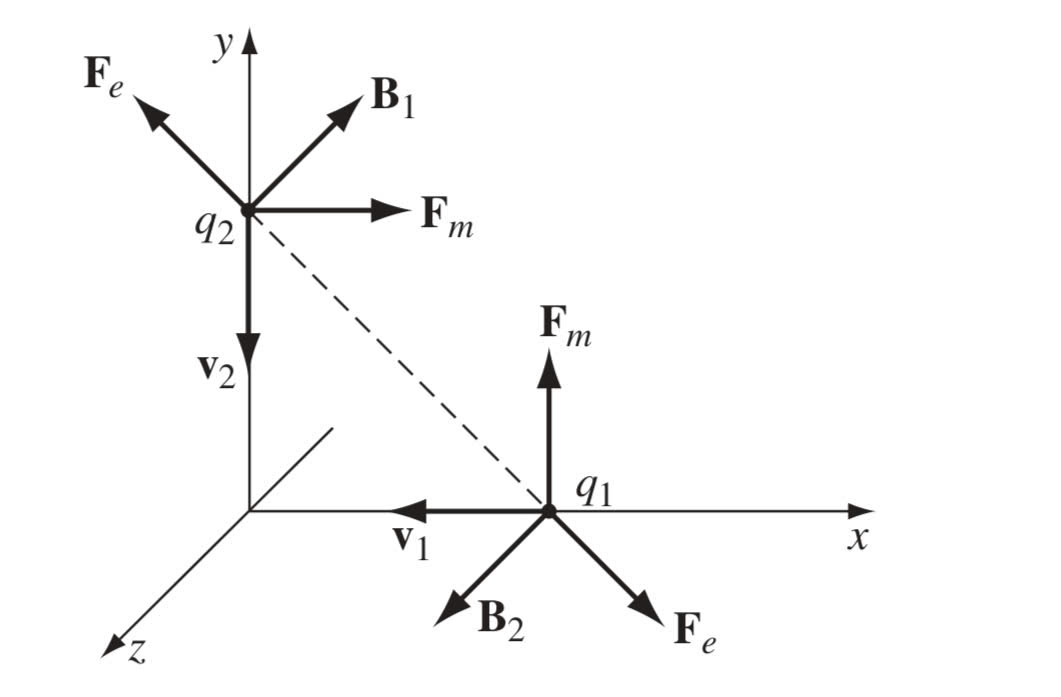
\includegraphics[width=7cm, height=5cm]{Slides/Figure/thirdlawinelectromagne.jpg}
        \caption{Định luật III Newton bị vi phạm}
    \end{figure}
        \end{column}
        \begin{column}{0.5\textwidth}
            Phương trình động lực học trong trường hợp này
            \[\frac{d}{dt}\left(\mathbf{p}+\int_{\mathcal{V}}c^{-2}~\mathbf{S}d\tau\right)=\oint_{\mathcal{S}}\overleftrightarrow{\mathbf{T}}\cdot d\mathbf{a},\]
            với \(\mathbf{S}=\mu_0^{-1}~\mathbf{E}\times\mathbf{B}\) gọi là vector Poynting. \newline Mật độ động lượng của trường được định nghĩa là 
            \[\mathbf{g}=c^{-2}~\mathbf{S}.\]
            Tích phân \(\int_{\mathcal{V}}\mathbf{g}~d\tau\) được gọi là \emph{động lượng được lưu trữ trong trường điện từ}.
        \end{column}
    \end{columns}
\end{frame}





 